% !TeX program = xelatex
% !TeX encoding = UTF-8
\documentclass[UTF8]{standalone}
\usepackage{amsmath,fourier,ctex,tikz}
\begin{document}
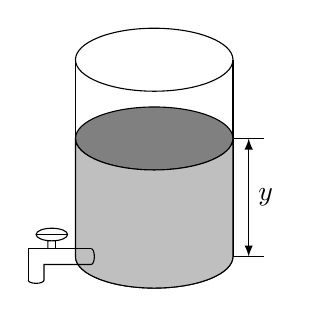
\begin{tikzpicture}
	\draw (1,0) arc [start angle=0, end angle=-180, x radius=1, y radius=0.4];
	\draw (-1,0) -- ++ (0,2.5);
	\draw (1,0) -- ++ (0,2.5);
	\draw (1,2.5) arc [start angle=0, end angle=360, x radius=1, y radius=0.4];
	\draw (1,0) -- ++ (0.4,0);
	\draw (1,1.5) -- ++ (0.4,0);
	\draw[latex-latex] (1.2,0) -- node[right] {$y$} ++ (0,1.5);
	\filldraw[fill=gray,draw=black] (1,1.5) arc [start angle=0, end angle=360, x radius=1, y radius=0.4];
	\fill[fill=lightgray,draw=black] (1,0) -- (1,1.5) -- (1,1.5) arc [start angle=0, end angle=-180, x radius=1, y radius=0.4] -- (-1,0) -- (-1,0) arc [start angle=-180, end angle=0, x radius=1, y radius=0.4] -- (1,0);
	\draw (-0.8,-0.1) arc [start angle=-90, end angle=90, x radius=0.04, y radius=0.1];
	\draw (-0.8,0.1) -- ++ (-0.8,0) -- ++ (0,-0.4);
	\draw (-0.8,-0.1) -- ++ (-0.6,0) -- ++ (0,-0.2) arc [start angle=0, end angle=-180, x radius=0.1, y radius=0.04];
	\draw (-1.35,0.1) -- ++ (0,0.1) ++ (0.05,0) arc [start angle=-90, end angle=270, x radius=0.2, y radius=0.08];
	\draw (-1.25,0.1) -- ++ (0,0.1);
	\draw (-1.5,0.28) -- ++ (0.4,0);
\end{tikzpicture}
\end{document}